
\documentclass[letterpaper,hide notes,xcolor={table,svgnames},pdftex,10pt]{beamer}
\def\showexamples{t}

\usecolortheme{crane}
\setbeamertemplate{navigation symbols}{}

\usetheme{MyPittsburgh}
\usepackage{hyperref}
\usepackage{graphicx,xspace}
\usepackage[normalem]{ulem}
\usepackage{multicol}
\usepackage{amsmath,amssymb,amsthm,graphicx,xspace}
\newcommand\SF[1]{$\bigstar$\footnote{SF: #1}}

\usepackage[sfdefault,lf]{carlito}
\usepackage[T1]{fontenc}
\usepackage[scaled]{beramono}
\usepackage{tikzpagenodes}
\newcommand{\Rplus}{\protect\hspace{-.1em}\protect\raisebox{.35ex}{\small{\small\textbf{+}}}}
\newcommand{\Cpp}{\mbox{C\Rplus\Rplus}\xspace}

\newcounter{tmpnumSlide}
\newcounter{tmpnumNote}

\newcommand\mnote[1]{%
	\addtocounter{tmpnumSlide}{1}
	\ifdefined\showcues {~\tiny\fbox{\arabic{tmpnumSlide}}}\fi
	\note{\setlength{\parskip}{1ex}\addtocounter{tmpnumNote}{1}\textbf{\Large \arabic{tmpnumNote}:} {#1\par}}}

\newcommand\mmnote[1]{\note{\setlength{\parskip}{1ex}#1\par}}


\newcommand\mquestion[2]{{~\color{red}\fbox{?}}\note{\setlength{\parskip}{1ex}\par{\Large \textbf{?}} #1} \note{\setlength{\parskip}{1ex}\par{\Large \textbf{A}} #2\par}\ifdefined \presentationonly \pause \fi}

\newcommand\blackboard[1]{%
	\ifdefined   \showblackboard
		{#1}
	\else {\begin{center} \fbox{\colorbox{blue!30}{%
						\begin{minipage}{.95\linewidth}%
							\hspace{\stretch{1}} Some space intentionally left blank; done at the blackboard.%
						\end{minipage}}}\end{center}}%
	\fi%
}

\usepackage{listings}
\lstset{%
	keywordstyle=\bfseries,
	aboveskip=15pt,
	belowskip=15pt,
	captionpos=b,
	identifierstyle=\ttfamily,
	frame=lines,
	numbers=left, basicstyle=\scriptsize, numberstyle=\tiny, stepnumber=0, numbersep=2pt}

\usepackage{siunitx}
\newcommand\sius[1]{\num[group-separator = {,}]{#1}\si{\micro\second}}
\newcommand\sims[1]{\num[group-separator = {,}]{#1}\si{\milli\second}}
\newcommand\sins[1]{\num[group-separator = {,}]{#1}\si{\nano\second}}
\sisetup{group-separator = {,}, group-digits = true}

%% -------------------- tikz --------------------
\usepackage{tikz}
\usetikzlibrary{positioning}
\usetikzlibrary{arrows,backgrounds,automata,decorations.shapes,decorations.pathmorphing,decorations.markings,decorations.text}

\tikzstyle{place}=[circle,draw=blue!50,fill=blue!20,thick, inner sep=0pt,minimum size=6mm]
\tikzstyle{transition}=[rectangle,draw=black!50,fill=black!20,thick, inner sep=0pt,minimum size=4mm]

\tikzstyle{block}=[rectangle,draw=black, thick, inner sep=5pt]
\tikzstyle{bullet}=[circle,draw=black, fill=black, thin, inner sep=2pt]

\tikzstyle{pre}=[<-,shorten <=1pt,>=stealth',semithick]
\tikzstyle{post}=[->,shorten >=1pt,>=stealth',semithick]
\tikzstyle{bi}=[<->,shorten >=1pt,shorten <=1pt, >=stealth',semithick]

\tikzstyle{mut}=[-,>=stealth',semithick]

\tikzstyle{treereset}=[dashed,->, shorten >=1pt,>=stealth',thin]

\usepackage{ifmtarg}
\usepackage{xifthen}
\makeatletter
% new counter to now which frame it is within the sequence
\newcounter{multiframecounter}
% initialize buffer for previously used frame title
\gdef\lastframetitle{\textit{undefined}}
% new environment for a multi-frame
\newenvironment{multiframe}[1][]{%
	\ifthenelse{\isempty{#1}}{%
		% if no frame title was set via optional parameter,
		% only increase sequence counter by 1
		\addtocounter{multiframecounter}{1}%
	}{%
		% new frame title has been provided, thus
		% reset sequence counter to 1 and buffer frame title for later use
		\setcounter{multiframecounter}{1}%
		\gdef\lastframetitle{#1}%
	}%
	% start conventional frame environment and
	% automatically set frame title followed by sequence counter
	\begin{frame}%
		\frametitle{\lastframetitle~{\normalfont(\arabic{multiframecounter})}}%
		}{%
	\end{frame}%
}
\makeatother

\makeatletter
\newdimen\tu@tmpa%
\newdimen\ydiffl%
\newdimen\xdiffl%
\newcommand\ydiff[2]{%
	\coordinate (tmpnamea) at (#1);%
	\coordinate (tmpnameb) at (#2);%
	\pgfextracty{\tu@tmpa}{\pgfpointanchor{tmpnamea}{center}}%
	\pgfextracty{\ydiffl}{\pgfpointanchor{tmpnameb}{center}}%
	\advance\ydiffl by -\tu@tmpa%
}
\newcommand\xdiff[2]{%
	\coordinate (tmpnamea) at (#1);%
	\coordinate (tmpnameb) at (#2);%
	\pgfextractx{\tu@tmpa}{\pgfpointanchor{tmpnamea}{center}}%
	\pgfextractx{\xdiffl}{\pgfpointanchor{tmpnameb}{center}}%
	\advance\xdiffl by -\tu@tmpa%
}
\makeatother
\newcommand{\copyrightbox}[3][r]{%
	\begin{tikzpicture}%
		\node[inner sep=0pt,minimum size=2em](ciimage){#2};
		\usefont{OT1}{phv}{n}{n}\fontsize{4}{4}\selectfont
		\ydiff{ciimage.south}{ciimage.north}
		\xdiff{ciimage.west}{ciimage.east}
		\ifthenelse{\equal{#1}{r}}{%
			\node[inner sep=0pt,right=1ex of ciimage.south east,anchor=north west,rotate=90]%
			{\raggedleft\color{black!50}\parbox{\the\ydiffl}{\raggedright{}#3}};%
		}{%
			\ifthenelse{\equal{#1}{l}}{%
				\node[inner sep=0pt,right=1ex of ciimage.south west,anchor=south west,rotate=90]%
				{\raggedleft\color{black!50}\parbox{\the\ydiffl}{\raggedright{}#3}};%
			}{%
				\node[inner sep=0pt,below=1ex of ciimage.south west,anchor=north west]%
				{\raggedleft\color{black!50}\parbox{\the\xdiffl}{\raggedright{}#3}};%
			}
		}
	\end{tikzpicture}
}


%% --------------------

%\usepackage[excludeor]{everyhook}
%\PushPreHook{par}{\setbox0=\lastbox\llap{MUH}}\box0}

%\vspace*{\stretch{1}

%\setbox0=\lastbox \llap{\textbullet\enskip}\box0}

\setlength{\parskip}{\fill}

\newcommand\noskips{\setlength{\parskip}{1ex}}
\newcommand\doskips{\setlength{\parskip}{\fill}}

\newcommand\xx{\par\vspace*{\stretch{1}}\par}
\newcommand\xxs{\par\vspace*{2ex}\par}
\newcommand\tuple[1]{\langle #1 \rangle}
\newcommand\code[1]{{\sf \footnotesize #1}}
\newcommand\ex[1]{\uline{Example:} \ifdefined \presentationonly \pause \fi
	\ifdefined\showexamples#1\xspace\else{\uline{\hspace*{2cm}}}\fi}

\newcommand\ceil[1]{\lceil #1 \rceil}


\AtBeginSection[]
{
	\begin{frame}
		\frametitle{Outline}
		\tableofcontents[currentsection]
	\end{frame}
}



\pgfdeclarelayer{edgelayer}
\pgfdeclarelayer{nodelayer}
\pgfsetlayers{edgelayer,nodelayer,main}

\tikzstyle{none}=[inner sep=0pt]
\tikzstyle{rn}=[circle,fill=Red,draw=Black,line width=0.8 pt]
\tikzstyle{gn}=[circle,fill=Lime,draw=Black,line width=0.8 pt]
\tikzstyle{yn}=[circle,fill=Yellow,draw=Black,line width=0.8 pt]
\tikzstyle{empty}=[circle,fill=White,draw=Black]
\tikzstyle{bw} = [rectangle, draw, fill=blue!20,
text width=4em, text centered, rounded corners, minimum height=2em]

\newcommand{\CcNote}[1]{% longname
	This work is licensed under the \textit{Creative Commons #1 3.0 License}.%
}
\newcommand{\CcImageBy}[1]{%
	\includegraphics[scale=#1]{creative_commons/cc_by_30.pdf}%
}
\newcommand{\CcImageSa}[1]{%
	\includegraphics[scale=#1]{creative_commons/cc_sa_30.pdf}%
}
\newcommand{\CcImageNc}[1]{%
	\includegraphics[scale=#1]{creative_commons/cc_nc_30.pdf}%
}
\newcommand{\CcGroupBySa}[2]{% zoom, gap
	\CcImageBy{#1}\hspace*{#2}\CcImageNc{#1}\hspace*{#2}\CcImageSa{#1}%
}
\newcommand{\CcLongnameByNcSa}{Attribution-NonCommercial-ShareAlike}

\newenvironment{changemargin}[1]{% 
	\begin{list}{}{% 
		\setlength{\topsep}{0pt}% 
		\setlength{\leftmargin}{#1}% 
		\setlength{\rightmargin}{1em}
		\setlength{\listparindent}{\parindent}% 
		\setlength{\itemindent}{\parindent}% 
		      \setlength{\parsep}{\parskip}% 
		      }% 
		\item[]}{\end{list}}




\title{Lecture 21 --- Scheduling Algorithms}

\author{Jeff Zarnett \\ \small \texttt{jzarnett@uwaterloo.ca}}
\institute{Department of Electrical and Computer Engineering \\
  University of Waterloo}
\date{\today}


\begin{document}

\begin{frame}
  \titlepage

 \end{frame}



\begin{frame}
\frametitle{Scheduling Algorithms}

Earlier we saw one example of a simple scheduling algorithm. 

Always choose the highest priority (non-blocked) task, and execute it. 

 \end{frame}



\begin{frame}
\frametitle{Scheduling Algorithms}


There are many options:
\begin{enumerate}
	\item Highest Priority, Period
	\item First-Come, First-Served
	\item Round Robin
	\item Shortest Process Next
	\item Shortest Job First
	\item Smallest Remaining Time
	\item Highest Response Ratio Next
	\item Multilevel Queue (Feedback)
	\item Guaranteed Scheduling
	\item Lottery
\end{enumerate}


\end{frame}

\begin{frame}
\frametitle{Scheduling Criteria}

Data about each process to be used in making decisions about scheduling:

\begin{enumerate}
	\item The time spent waiting to run.
	\item The time spent executing.
	\item The total time of execution.
\end{enumerate}

Desktop OSes do not ask users for estimates, but supercomputers might.

\end{frame}

\begin{frame}
\frametitle{Highest Priority, Period}

\begin{center}
	
\includegraphics[width=\textwidth]{images/geringverdiener.jpg}
\end{center}

\end{frame}

\begin{frame}
\frametitle{Highest Priority, Period}

Implementing this is not difficult; priority queues (one for each priority level).
 
If the process's priority is changed, move it to its new home. 

We might have a priority heap, or just one big linked list or array that we keep sorted by priority.

\end{frame}



\begin{frame}
\frametitle{Highest Priority, Period}


The flaw in this has already been identified: it is vulnerable to starvation. 

A process of relatively low priority may never get the chance to run, because there is always something better to do right now. 

Software projects may have bug reports open for years on end because they are never important enough to be addressed.

\end{frame}

\begin{frame}
\frametitle{Highest Priority, Period}

In some systems this is a desirable property. 

It does not fulfill all short term scheduling criteria (response time, fairness). 

It may be suitable for life-and-safety-critical systems.

Example: control a robot arm, to prevent a situation where the robot arm goes through the wall and the building falls down and you're dead.


\end{frame}


\begin{frame}
\frametitle{First-Come, First-Served}

\begin{center}
	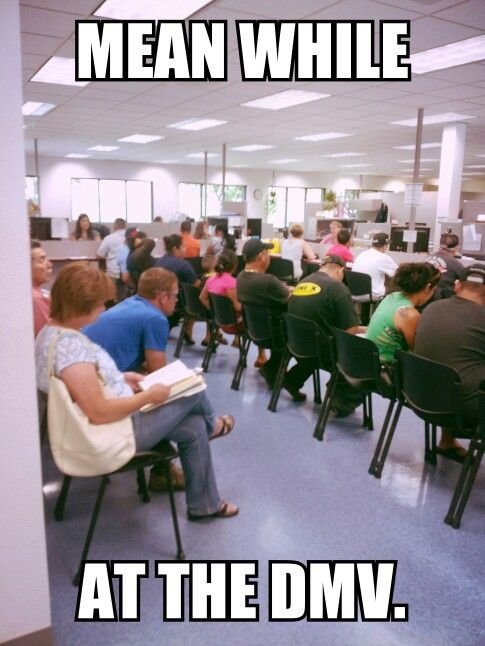
\includegraphics[width=0.5\textwidth]{images/dmv.jpg}
\end{center}


\end{frame}


\begin{frame}
\frametitle{First-Come, First-Served}

This is an obvious algorithm that is simple to implement. 

Whichever process requests the CPU first gets the CPU first. 

Just imagine a queue of processes in which all processes are equal. 


\end{frame}


\begin{frame}
\frametitle{First-Come, First-Served}


A process enters the queue at the back and whichever process is at the front will be dequeued and get to run.  

If the current process finishes or is blocked for some reason, the next ready process is selected. 


\end{frame}



\begin{frame}
\frametitle{First-Come, First-Served}

This is actually a simplification of the highest priority, period scheme.

It ignores priority altogether. 

All processes get a chance to run eventually; low priority processes don't starve.


\end{frame}

\begin{frame}
\frametitle{FCFS: Wait Times}

FCFS can result in some undesirable outcomes. 

The average waiting time for processes might vary wildly. 

Consider if we have three processes, $P_{1}$, $P_{2}$, and $P_{3}$. 

$P_{1}$ needs 24 units of CPU time; $P_{2}$ and $P_{3}$ require 3 units each.

\end{frame}

\begin{frame}
\frametitle{FCFS: Wait Times}

\begin{center}
	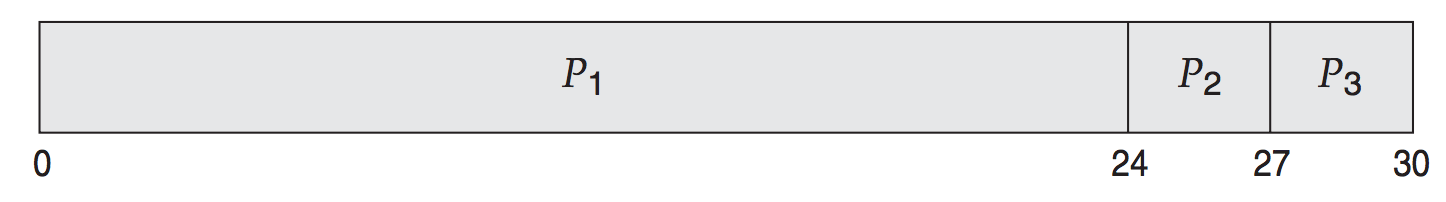
\includegraphics[width=0.9\textwidth]{images/fcfs-1.png}
\end{center}

Total time: 30 units. Average completion time: 27 units.
\begin{center}
	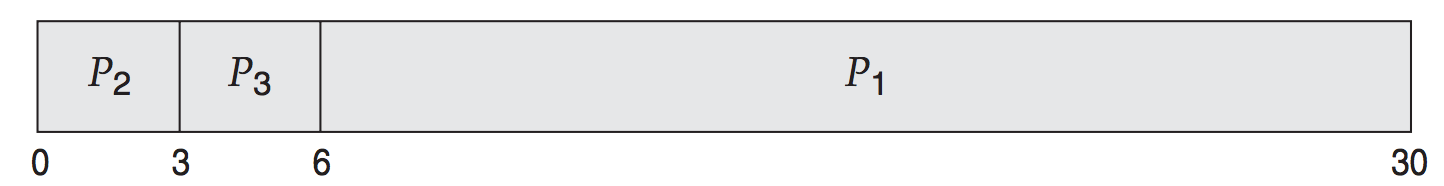
\includegraphics[width=0.9\textwidth]{images/fcfs-2.png}
\end{center}

Total time: 30 units. Average completion time: 13 units.

\end{frame}

\begin{frame}
\frametitle{FCFS: Favouritism}

FCFS also tends to favour CPU-Bound processes. 

When a CPU-Bound process is running, the I/O bound processes must wait in the queue like everybody else. 

This might lead to inefficient use of the resources; disk is slow so we would like to keep it busy at all times. 

With FCFS, however, the I/O devices are likely to suffer idle periods.

\end{frame}

\begin{frame}
\frametitle{FCFS: Preemption}

The FCFS algorithm as it is generally described, is non-preemptive.

A process that gets selected from the front of the queue runs until there is a reason to make the swap. 

So in theory, one process could monopolize the CPU (remember that some people are jerks). 

If we modify FCFS with periodic preemption, then we get Round Robin.

\end{frame}


\begin{frame}
\frametitle{Round Robin}

\begin{center}
	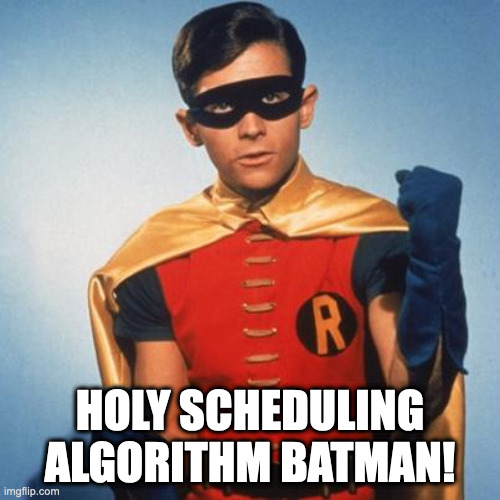
\includegraphics[width=0.5\textwidth]{images/roundrobin.jpg}
\end{center}


\end{frame}


\begin{frame}
\frametitle{Round Robin}

The idea of time slicing has already been introduced. 

Every $t$ units of time, a timer generates an interrupt that is the prompt to run the short-term scheduler. 

Time slicing itself can be combined with many of the strategies for choosing the next process, but when it is combined with FCFS we get Round Robin. 


\end{frame}

\begin{frame}
\frametitle{How Big of a Slice?}

The principal issue is: how big should $t$ be? 

If $t$ is too long, then processes may seem to be unresponsive while some other process has the CPU. 

Short processes may have to wait quite a while for their turn.

If $t$ is too short, the system spends a lot of time handling the clock interrupt and running the scheduling algorithm.


\end{frame}

\begin{frame}
\frametitle{How Big of a Slice?}

We could decide about the size of $t$ based on the patterns of the system. 

Suppose a typical process tends to run for $r$ time units before getting blocked.

It would be logical to choose $t$ such that it is slightly larger than $r$. 

\end{frame}

\begin{frame}
\frametitle{How Big of a Slice?}

If $t$ is smaller than $r$, processes will frequently be interrupted by the time slice. 

Processes that are going to use a lot of CPU will be split up over multiple time slices anyways, but it's frustrating if the process would take 1.1 time slices. 

If $t$ is larger than $r$, many processes will not run up against that time slice limit.

They will hopefully accomplish a useful chunk of work before getting blocked for I/O or some other reason. 

\end{frame}

\begin{frame}
\frametitle{Round Robin}

Round Robin tends to favour CPU-Bound processes. 

An I/O-Bound process spends a lot less time using the CPU. 

It runs for a short time, gets blocked on I/O, then when the I/O is finished, it goes back in the ready queue. 

So CPU-Bound processes are getting more of the CPU time.


\end{frame}


\begin{frame}
\frametitle{Virtual Round Robin}

\begin{center}
	
\includegraphics[width=0.75\textwidth]{images/virtualrobin.jpg}
\end{center}

\end{frame}



\begin{frame}
\frametitle{Virtual Round Robin}

Round Robin can be improved to Virtual Round Robin to address this. 

It works like Round Robin, but a process that gets unblocked after I/O gets higher priority.

Instead of just rejoining the general queue, there is an auxiliary queue for processes that were previously blocked on I/O.

\end{frame}

\begin{frame}
\frametitle{Virtual Round Robin}

When the scheduler is choosing a process to run, it takes them from the auxiliary queue if possible. 

If a process simply ran up against the time limit, it goes into the regular ready queue instead. 

If dispatched from the auxiliary queue, it runs for up to the as-yet-unused fraction of a slice.

\end{frame}

\begin{frame}
\frametitle{Virtual Round Robin}

\begin{center}
	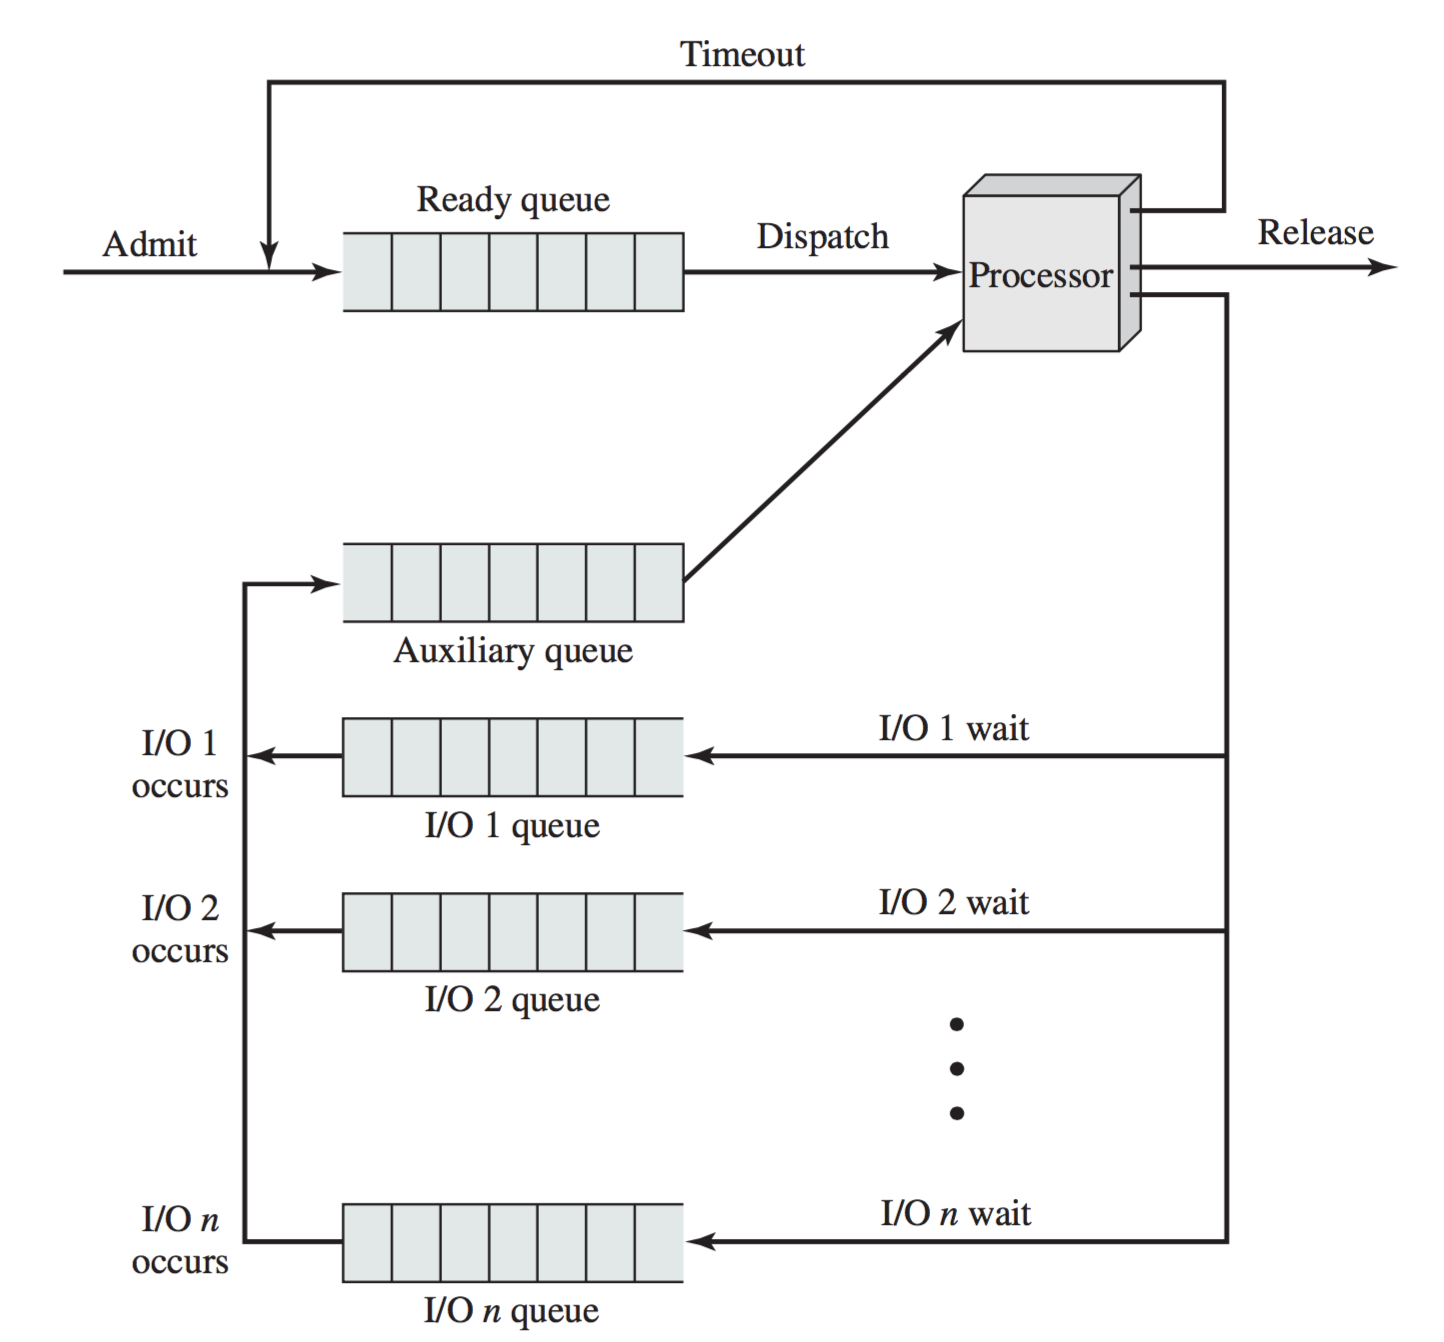
\includegraphics[width=0.65\textwidth]{images/virtual-round-robin.png}.
\end{center}


\end{frame}


\begin{frame}
\frametitle{Shortest Process Next}

\begin{center}
	
\includegraphics[width=0.65\textwidth]{images/quick-adventure.png}
\end{center}


\end{frame}


\begin{frame}
\frametitle{Shortest Process Next}

If some information is available about the total length of execution then we may wish to give priority to short processes. 


Average time to completion of a task was a lot lower when the shorter processes of $P_{2}$ and $P_{3}$ ran before $P_{1}$. 

This means we will get faster turnaround times and better responsiveness, but longer processes may be waiting an unpredictable amount of time.

\end{frame}

\begin{frame}
\frametitle{Shortest Process Next}

This is the sort of thing that used to happen in batch job processing on mainframes. 

The programmer was asked to give an estimate of the amount of time the program (e.g., compile) would run. 

If the programmer's estimate was too low, the program execution would be terminated early. 

If the programmer's estimate was too high, the job may never be scheduled to run, or at least, have to wait a very long time. 


\end{frame}

\begin{frame}
\frametitle{Shortest Process Next}


This might work, but you have noticed that the OS does not ask you, when you start a text editor, roughly how long you expect to be. 

Your boss on co-op may not be so accommodating. 

This is also a global assessment: how long the whole process takes. 

It might be better to worry about the length of CPU bursts and make decisions somewhat more locally...


\end{frame}


\begin{frame}
\frametitle{Shortest Job First}

\begin{center}
	
\includegraphics[width=0.5\textwidth]{images/quick-update.jpg}
\end{center}


\end{frame}


\begin{frame}
\frametitle{Shortest Job First}

This strategy, unfortunately, is not given quite the right name, but it's the common name for the scheme. 

We should call it ``shortest next CPU burst''.

Then again, the other sciences are not so good at naming things either... the Red Panda is not a Panda at all.

\begin{center}
	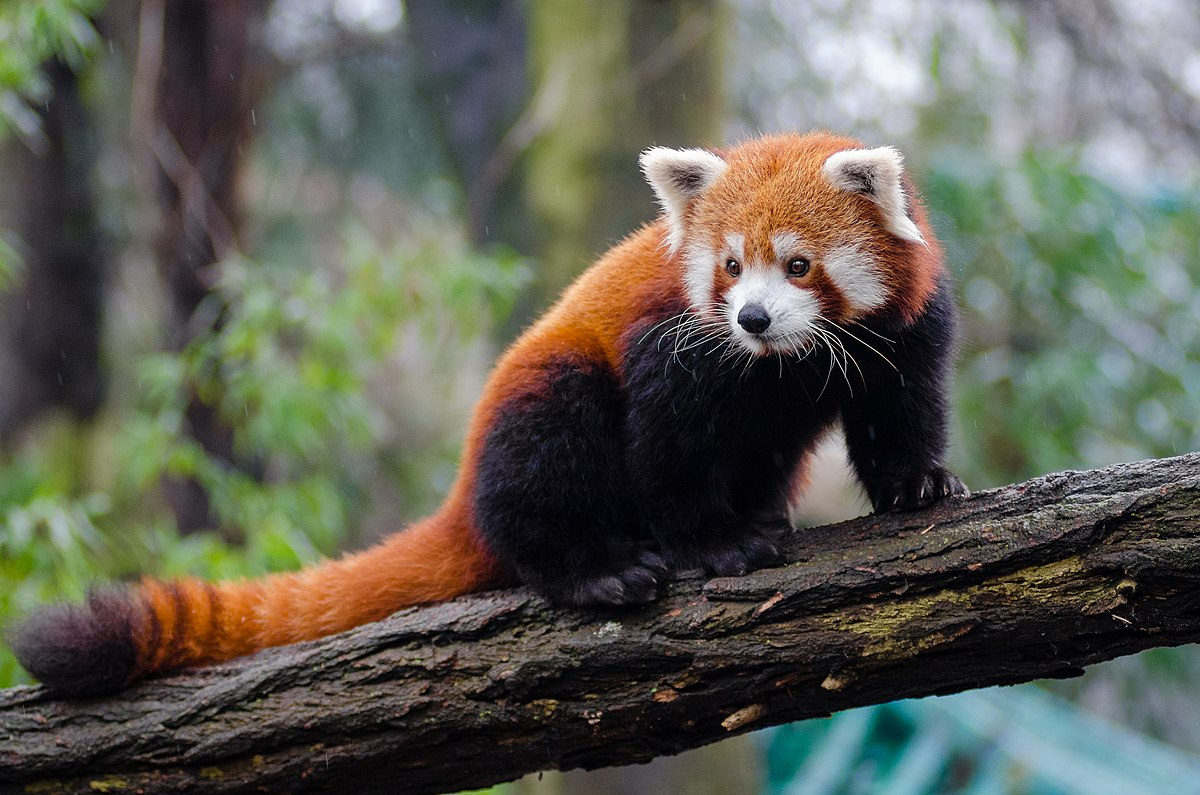
\includegraphics[width=0.4\textwidth]{images/redpanda.jpg}
\end{center}

\end{frame}


\begin{frame}
\frametitle{Shortest Job First}



Choose the process that is likely to have the smallest CPU burst. 

If two are the same, then FCFS can break the tie (or just choose randomly). 


\end{frame}

\begin{frame}
\frametitle{Smallest CPU Burst}

 

Imagine $P_{1}$ through $P_{4}$, whose predicted burst times are 6, 8, 7, and 3 respectively. 

We should schedule then such that the order would be $P_{4}, P_{1}, P_{3}, P_{2}$.

\begin{center}
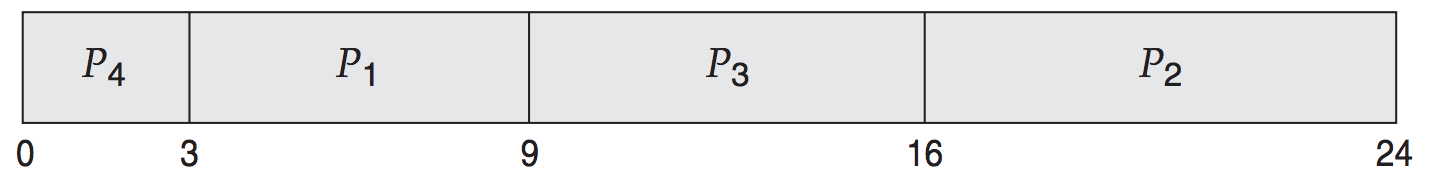
\includegraphics[width=0.7\textwidth]{images/sjf.png}
\end{center}

The average waiting time is $(3 + 16 + 9 + 0) / 4$ = 7 units of time. 

\end{frame}

\begin{frame}
\frametitle{Smallest CPU Burst}

This is significantly better than the FCFS scheduling. 

The algorithm is provably optimal in giving the minimum average waiting time for processes. 

Moving a short process up means it finishes faster, and that decreases its waiting time, while moving longer processes back increases their waiting time. 

Overall, this scheme is a net positive; the decreases outweigh the increases.

\end{frame}

\begin{frame}
\frametitle{Smallest CPU Burst}

The problem is predicting the CPU burst times. 

The best thing we may be able to do is gather information about the past and use that to guess about the future. 

\begin{center}
$S_{n+1} = \frac{1}{n}\displaystyle\sum_{i=1}^{n}T_{i}$
\end{center}

where:\\
\quad $T_{i}$ is the burst time for the $i$th instance of this process;\\
\quad $S_{i}$ is the predicted value for the $i$th instance; \\
\quad and $S_{1}$ is a guess at the first value.

\end{frame}

\begin{frame}
\frametitle{Estimating CPU Burst}

Instead of a sum each time, modify the equation to just update the value:

\begin{center}
$S_{n+1} = \frac{1}{n}T_{n} + \frac{n - 1}{n} S_{n}$
\end{center}

This routine gives each term in the summation equal weight of $\frac{1}{n}$. 

\end{frame}


\begin{frame}
\frametitle{Estimating CPU Burst}

Give greater weight to the more recent values: exponential averaging. 

Define a weighting factor $\alpha$, somewhere between 0 and 1, that determines how much weight the observations are given:

\begin{center}
$S_{n+1} = \alpha T_{n} + (1 - \alpha) S_{n}$
\end{center}

The larger the value of $\alpha$, the more the recent observations matter.

\end{frame}

\begin{frame}
\frametitle{Exponential Averaging}

\begin{center}
	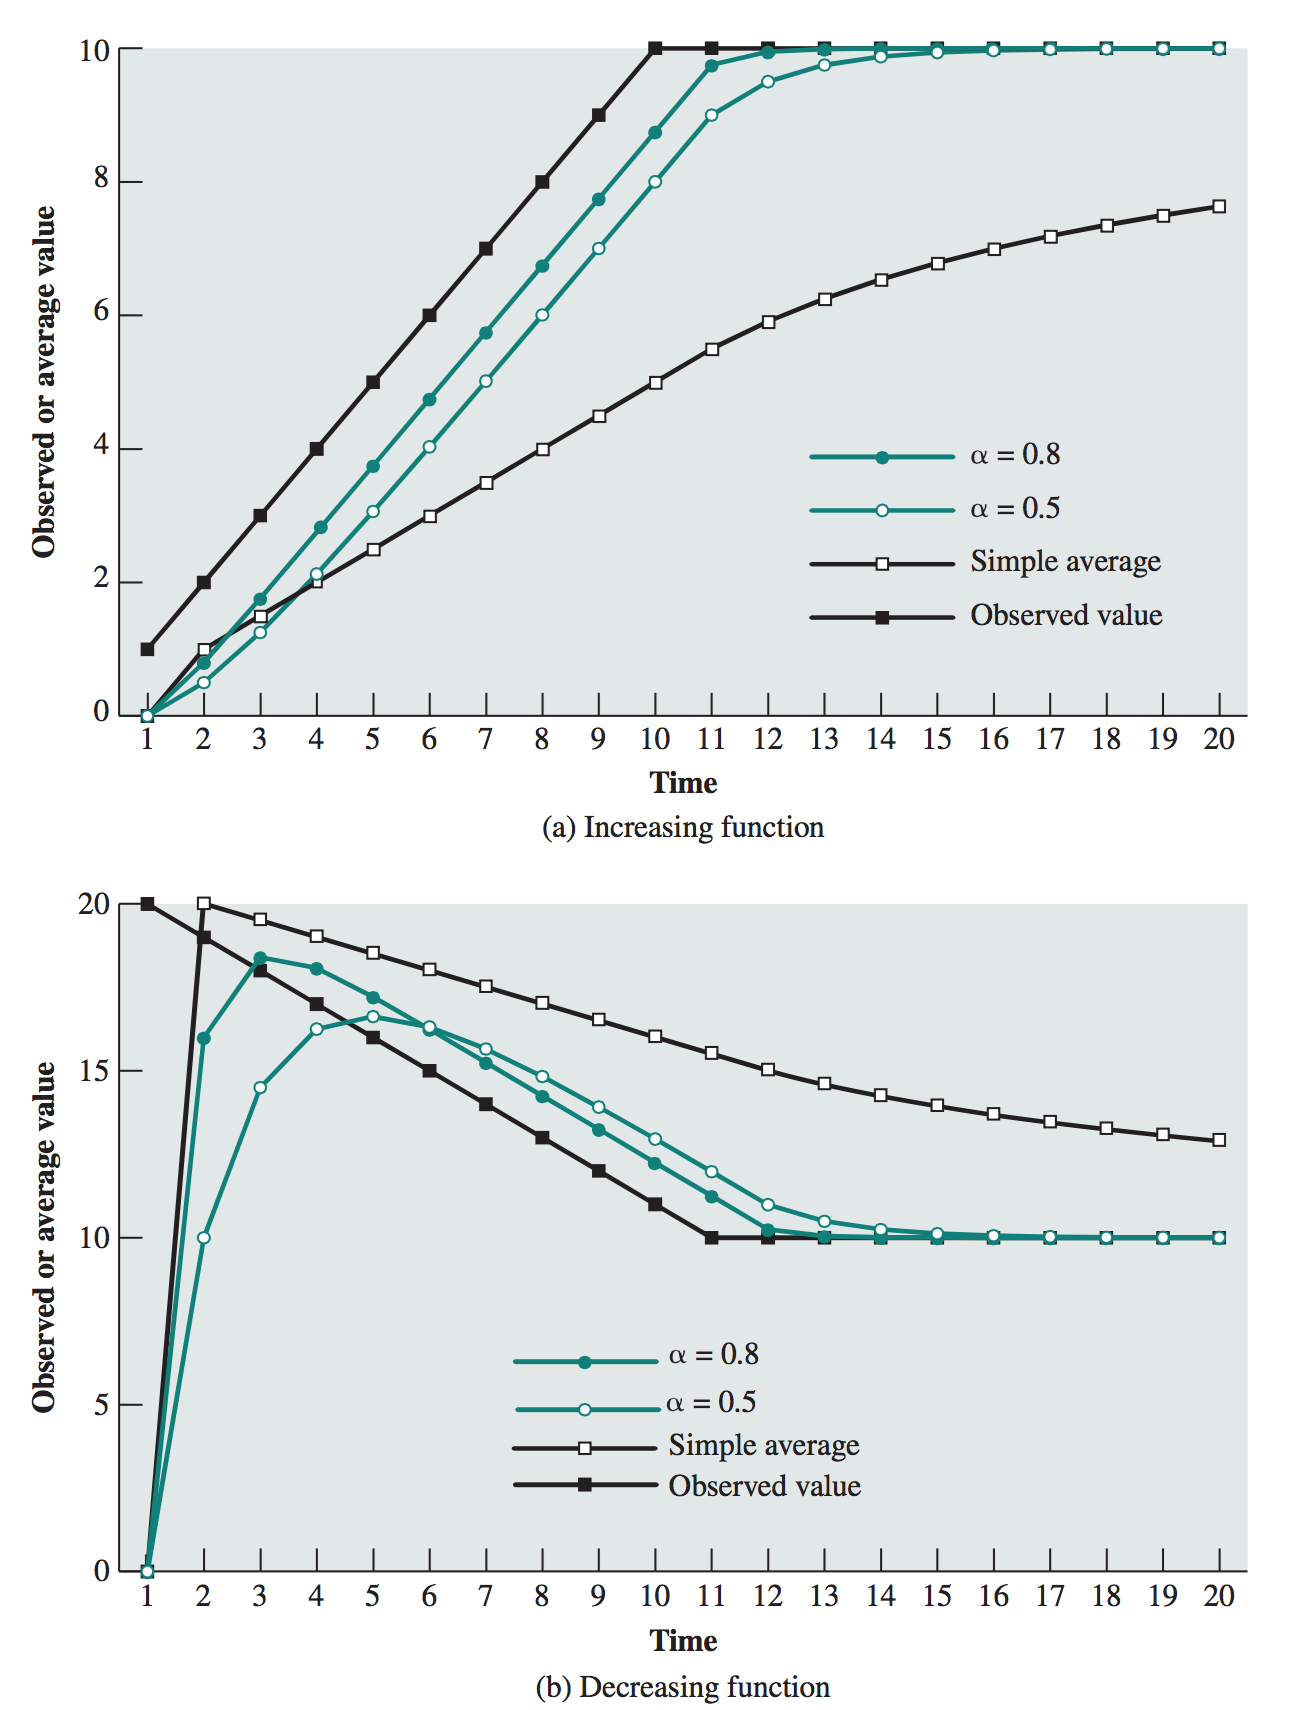
\includegraphics[width=0.5\textwidth]{images/exponential-averaging.png}
\end{center}

\end{frame}

\begin{frame}
\frametitle{Choosing a Starting Value}


We might give an estimate of $S_{1} = 0$ to start with, which gives new processes priority and a chance to get started. 

After they have started and run a bit, we will have some data. 

But first we have to give them a chance.

There is still a chance that longer processes will starve. 

If there is a constant stream of shorter processes, they will continue to get scheduled ahead of a long one...

\end{frame}

\begin{frame}
\frametitle{Predictions and CPU Burst}

\begin{center}
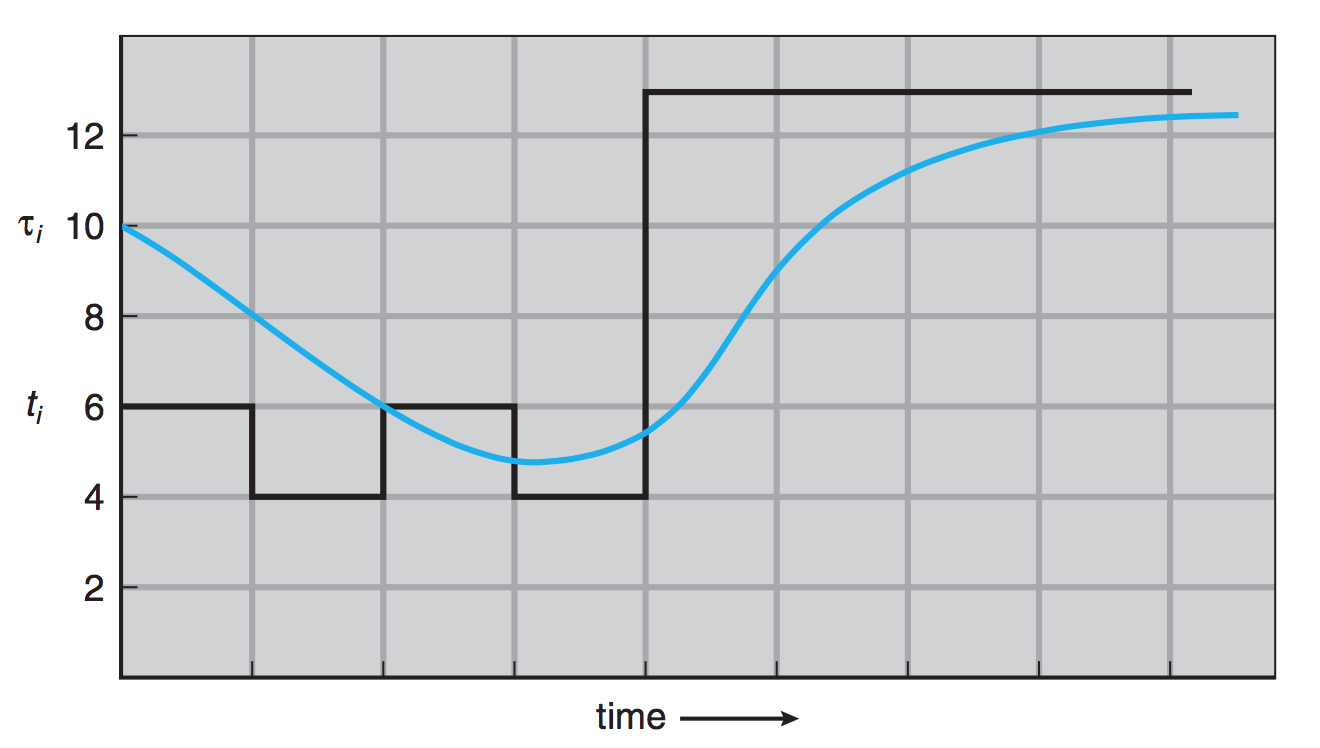
\includegraphics[width=\textwidth]{images/sjf-2.png}
\end{center}


\end{frame}


\begin{frame}
\frametitle{Shortest Remaining Time}

\begin{center}
	
\includegraphics[width=0.7\textwidth]{images/stay-on-target.jpg}
\end{center}


\end{frame}


\begin{frame}
\frametitle{Shortest Remaining Time}

Shortest remaining time is a modification of the preceding strategy, which allows for some additional preemption. 

When a new process is scheduled or an old one becomes unblocked, the scheduler will run.

It evaluates if the candidate has a shorter predicted running time than the currently-executing process. 

If so, then the candidate will displace the currently-executing one and start running right away.


\end{frame}

\begin{frame}
\frametitle{Shortest Remaining Time}

As with Shortest Process Next, there is a chance that long processes will starve because of a steady stream of shorter processes. 

For Short Job First, if we choose $S_{1}$ to be zero for new processes, it means they will always preempt the running process which may be undesirable.


\end{frame}

\begin{frame}
\frametitle{Shortest Remaining Time Slicing}

One advantage: we no longer need to have time slicing. 

Instead of interrupting the running process every $t$ units of time, the other interrupts will be the prompts to run the scheduler. 

Thus, the system does not spend any time handling the clock interrupts, which will be a performance increase. 

Handling the clock interrupt is not expensive, but even an inexpensive operation, done a million times, will eventually add up...


\end{frame}



\begin{frame}
\frametitle{Batch and Interactive}

So far the scheduling routines we have looked at are more suitable to batch processing systems than to interactive desktop systems. 

The remaining scheduling algorithms in the list will look a lot more like what we expect to see on our laptops and phones...


\end{frame}

\end{document}

